\documentclass[1p]{elsarticle_modified}
%\bibliographystyle{elsarticle-num}

%\usepackage[colorlinks]{hyperref}
%\usepackage{abbrmath_seonhwa} %\Abb, \Ascr, \Acal ,\Abf, \Afrak
\usepackage{amsfonts}
\usepackage{amssymb}
\usepackage{amsmath}
\usepackage{amsthm}
\usepackage{scalefnt}
\usepackage{amsbsy}
\usepackage{kotex}
\usepackage{caption}
\usepackage{subfig}
\usepackage{color}
\usepackage{graphicx}
\usepackage{xcolor} %% white, black, red, green, blue, cyan, magenta, yellow
\usepackage{float}
\usepackage{setspace}
\usepackage{hyperref}

\usepackage{tikz}
\usetikzlibrary{arrows}

\usepackage{multirow}
\usepackage{array} % fixed length table
\usepackage{hhline}

%%%%%%%%%%%%%%%%%%%%%
\makeatletter
\renewcommand*\env@matrix[1][\arraystretch]{%
	\edef\arraystretch{#1}%
	\hskip -\arraycolsep
	\let\@ifnextchar\new@ifnextchar
	\array{*\c@MaxMatrixCols c}}
\makeatother %https://tex.stackexchange.com/questions/14071/how-can-i-increase-the-line-spacing-in-a-matrix
%%%%%%%%%%%%%%%

\usepackage[normalem]{ulem}

\newcommand{\msout}[1]{\ifmmode\text{\sout{\ensuremath{#1}}}\else\sout{#1}\fi}
%SOURCE: \msout is \stkout macro in https://tex.stackexchange.com/questions/20609/strikeout-in-math-mode

\newcommand{\cancel}[1]{
	\ifmmode
	{\color{red}\msout{#1}}
	\else
	{\color{red}\sout{#1}}
	\fi
}

\newcommand{\add}[1]{
	{\color{blue}\uwave{#1}}
}

\newcommand{\replace}[2]{
	\ifmmode
	{\color{red}\msout{#1}}{\color{blue}\uwave{#2}}
	\else
	{\color{red}\sout{#1}}{\color{blue}\uwave{#2}}
	\fi
}

\newcommand{\Sol}{\mathcal{S}} %segment
\newcommand{\D}{D} %diagram
\newcommand{\A}{\mathcal{A}} %arc


%%%%%%%%%%%%%%%%%%%%%%%%%%%%%5 test

\def\sl{\operatorname{\textup{SL}}(2,\Cbb)}
\def\psl{\operatorname{\textup{PSL}}(2,\Cbb)}
\def\quan{\mkern 1mu \triangleright \mkern 1mu}

\theoremstyle{definition}
\newtheorem{thm}{Theorem}[section]
\newtheorem{prop}[thm]{Proposition}
\newtheorem{lem}[thm]{Lemma}
\newtheorem{ques}[thm]{Question}
\newtheorem{cor}[thm]{Corollary}
\newtheorem{defn}[thm]{Definition}
\newtheorem{exam}[thm]{Example}
\newtheorem{rmk}[thm]{Remark}
\newtheorem{alg}[thm]{Algorithm}

\newcommand{\I}{\sqrt{-1}}
\begin{document}

%\begin{frontmatter}
%
%\title{Boundary parabolic representations of knots up to 8 crossings}
%
%%% Group authors per affiliation:
%\author{Yunhi Cho} 
%\address{Department of Mathematics, University of Seoul, Seoul, Korea}
%\ead{yhcho@uos.ac.kr}
%
%
%\author{Seonhwa Kim} %\fnref{s_kim}}
%\address{Center for Geometry and Physics, Institute for Basic Science, Pohang, 37673, Korea}
%\ead{ryeona17@ibs.re.kr}
%
%\author{Hyuk Kim}
%\address{Department of Mathematical Sciences, Seoul National University, Seoul 08826, Korea}
%\ead{hyukkim@snu.ac.kr}
%
%\author{Seokbeom Yoon}
%\address{Department of Mathematical Sciences, Seoul National University, Seoul, 08826,  Korea}
%\ead{sbyoon15@snu.ac.kr}
%
%\begin{abstract}
%We find all boundary parabolic representation of knots up to 8 crossings.
%
%\end{abstract}
%\begin{keyword}
%    \MSC[2010] 57M25 
%\end{keyword}
%
%\end{frontmatter}

%\linenumbers
%\tableofcontents
%
\newcommand\colored[1]{\textcolor{white}{\rule[-0.35ex]{0.8em}{1.4ex}}\kern-0.8em\color{red} #1}%
%\newcommand\colored[1]{\textcolor{white}{ #1}\kern-2.17ex	\textcolor{white}{ #1}\kern-1.81ex	\textcolor{white}{ #1}\kern-2.15ex\color{red}#1	}

{\Large $\underline{12a_{0493}~(K12a_{0493})}$}

\setlength{\tabcolsep}{10pt}
\renewcommand{\arraystretch}{1.6}
\vspace{1cm}\begin{tabular}{m{100pt}>{\centering\arraybackslash}m{274pt}}
\multirow{5}{120pt}{
	\centering
	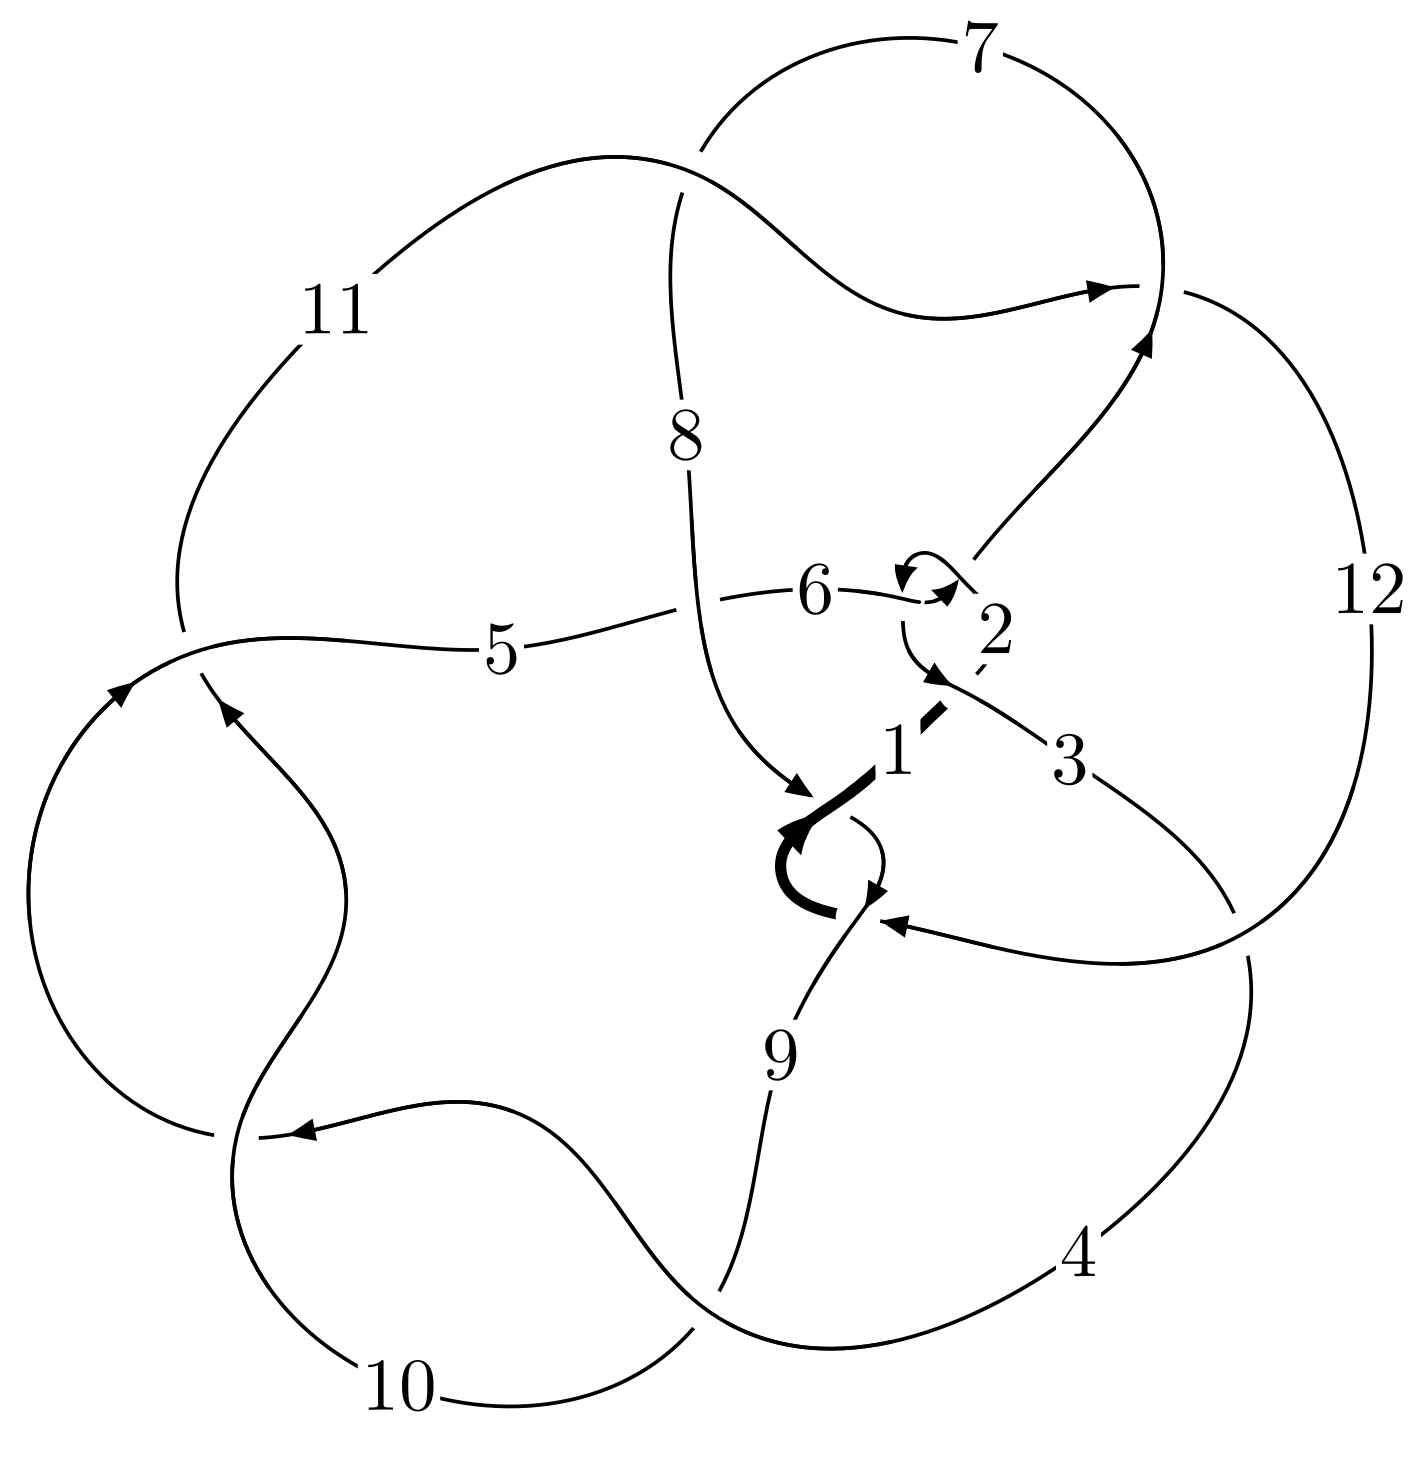
\includegraphics[width=112pt]{../../../GIT/diagram.site/Diagrams/png/1294_12a_0493.png}\\
\ \ \ A knot diagram\footnotemark}&
\allowdisplaybreaks
\textbf{Linearized knot diagam} \\
\cline{2-2}
 &
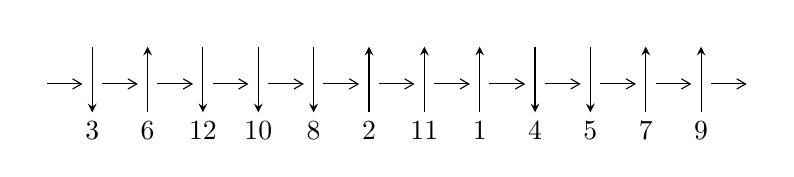
\begin{tikzpicture}[x=20pt, y=17pt]
	% nodes
	\node (C0) at (0, 0) {};
	\node (C1) at (1, 0) {};
	\node (C1U) at (1, +1) {};
	\node (C1D) at (1, -1) {3};

	\node (C2) at (2, 0) {};
	\node (C2U) at (2, +1) {};
	\node (C2D) at (2, -1) {6};

	\node (C3) at (3, 0) {};
	\node (C3U) at (3, +1) {};
	\node (C3D) at (3, -1) {12};

	\node (C4) at (4, 0) {};
	\node (C4U) at (4, +1) {};
	\node (C4D) at (4, -1) {10};

	\node (C5) at (5, 0) {};
	\node (C5U) at (5, +1) {};
	\node (C5D) at (5, -1) {8};

	\node (C6) at (6, 0) {};
	\node (C6U) at (6, +1) {};
	\node (C6D) at (6, -1) {2};

	\node (C7) at (7, 0) {};
	\node (C7U) at (7, +1) {};
	\node (C7D) at (7, -1) {11};

	\node (C8) at (8, 0) {};
	\node (C8U) at (8, +1) {};
	\node (C8D) at (8, -1) {1};

	\node (C9) at (9, 0) {};
	\node (C9U) at (9, +1) {};
	\node (C9D) at (9, -1) {4};

	\node (C10) at (10, 0) {};
	\node (C10U) at (10, +1) {};
	\node (C10D) at (10, -1) {5};

	\node (C11) at (11, 0) {};
	\node (C11U) at (11, +1) {};
	\node (C11D) at (11, -1) {7};

	\node (C12) at (12, 0) {};
	\node (C12U) at (12, +1) {};
	\node (C12D) at (12, -1) {9};
	\node (C13) at (13, 0) {};

	% arrows
	\draw[->,>={angle 60}]
	(C0) edge (C1) (C1) edge (C2) (C2) edge (C3) (C3) edge (C4) (C4) edge (C5) (C5) edge (C6) (C6) edge (C7) (C7) edge (C8) (C8) edge (C9) (C9) edge (C10) (C10) edge (C11) (C11) edge (C12) (C12) edge (C13) ;	\draw[->,>=stealth]
	(C1U) edge (C1D) (C2D) edge (C2U) (C3U) edge (C3D) (C4U) edge (C4D) (C5U) edge (C5D) (C6D) edge (C6U) (C7D) edge (C7U) (C8D) edge (C8U) (C9U) edge (C9D) (C10U) edge (C10D) (C11D) edge (C11U) (C12D) edge (C12U) ;
	\end{tikzpicture} \\
\hhline{~~} \\& 
\textbf{Solving Sequence} \\ \cline{2-2} 
 &
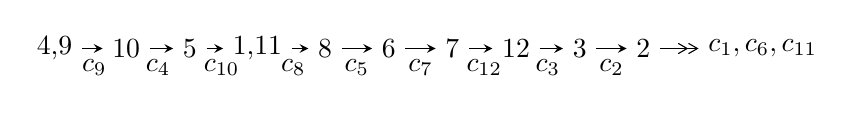
\begin{tikzpicture}[x=23pt, y=7pt]
	% node
	\node (A0) at (-1/8, 0) {4,9};
	\node (A1) at (1, 0) {10};
	\node (A2) at (2, 0) {5};
	\node (A3) at (49/16, 0) {1,11};
	\node (A4) at (33/8, 0) {8};
	\node (A5) at (41/8, 0) {6};
	\node (A6) at (49/8, 0) {7};
	\node (A7) at (57/8, 0) {12};
	\node (A8) at (65/8, 0) {3};
	\node (A9) at (73/8, 0) {2};
	\node (C1) at (1/2, -1) {$c_{9}$};
	\node (C2) at (3/2, -1) {$c_{4}$};
	\node (C3) at (5/2, -1) {$c_{10}$};
	\node (C4) at (29/8, -1) {$c_{8}$};
	\node (C5) at (37/8, -1) {$c_{5}$};
	\node (C6) at (45/8, -1) {$c_{7}$};
	\node (C7) at (53/8, -1) {$c_{12}$};
	\node (C8) at (61/8, -1) {$c_{3}$};
	\node (C9) at (69/8, -1) {$c_{2}$};
	\node (A10) at (11, 0) {$c_{1},c_{6},c_{11}$};

	% edge
	\draw[->,>=stealth]	
	(A0) edge (A1) (A1) edge (A2) (A2) edge (A3) (A3) edge (A4) (A4) edge (A5) (A5) edge (A6) (A6) edge (A7) (A7) edge (A8) (A8) edge (A9) ;
	\draw[->>,>={angle 60}]	
	(A9) edge (A10);
\end{tikzpicture} \\ 

\end{tabular} \\

\footnotetext{
The image of knot diagram is generated by the software ``\textbf{Draw programme}" developed by Andrew Bartholomew(\url{http://www.layer8.co.uk/maths/draw/index.htm\#Running-draw}), where we modified some parts for our purpose(\url{https://github.com/CATsTAILs/LinksPainter}).
}\phantom \\ \newline 
\centering \textbf{Ideals for irreducible components\footnotemark of $X_{\text{par}}$} 
 
\begin{align*}
I^u_{1}&=\langle 
-3.06014\times10^{50} u^{36}-1.13950\times10^{51} u^{35}+\cdots+1.85440\times10^{51} b-1.47847\times10^{52},\\
\phantom{I^u_{1}}&\phantom{= \langle  }-7.67176\times10^{51} u^{36}-2.81819\times10^{52} u^{35}+\cdots+1.48352\times10^{52} a-4.05802\times10^{53},\\
\phantom{I^u_{1}}&\phantom{= \langle  }u^{37}+3 u^{36}+\cdots+128 u-32\rangle \\
I^u_{2}&=\langle 
13 u^{27} a+13 u^{27}+\cdots+9 a-79,\;-126 u^{27} a+164 u^{27}+\cdots+105 a-202,\;u^{28}- u^{27}+\cdots-2 u-1\rangle \\
I^u_{3}&=\langle 
b-1,\;8 a^2-2 a u-8 a+u+3,\;u^2-2\rangle \\
I^u_{4}&=\langle 
b- u,\;3 a- u-1,\;u^2+1\rangle \\
\\
I^v_{1}&=\langle 
a,\;b+1,\;4 v^2-2 v+1\rangle \\
\end{align*}
\raggedright * 5 irreducible components of $\dim_{\mathbb{C}}=0$, with total 101 representations.\\
\footnotetext{All coefficients of polynomials are rational numbers. But the coefficients are sometimes approximated in decimal forms when there is not enough margin.}
\newpage
\renewcommand{\arraystretch}{1}
\centering \section*{I. $I^u_{1}= \langle -3.06\times10^{50} u^{36}-1.14\times10^{51} u^{35}+\cdots+1.85\times10^{51} b-1.48\times10^{52},\;-7.67\times10^{51} u^{36}-2.82\times10^{52} u^{35}+\cdots+1.48\times10^{52} a-4.06\times10^{53},\;u^{37}+3 u^{36}+\cdots+128 u-32 \rangle$}
\flushleft \textbf{(i) Arc colorings}\\
\begin{tabular}{m{7pt} m{180pt} m{7pt} m{180pt} }
\flushright $a_{4}=$&$\begin{pmatrix}0\\u\end{pmatrix}$ \\
\flushright $a_{9}=$&$\begin{pmatrix}1\\0\end{pmatrix}$ \\
\flushright $a_{10}=$&$\begin{pmatrix}1\\u^2\end{pmatrix}$ \\
\flushright $a_{5}=$&$\begin{pmatrix}- u\\- u^3+u\end{pmatrix}$ \\
\flushright $a_{1}=$&$\begin{pmatrix}0.517133 u^{36}+1.89967 u^{35}+\cdots-65.6808 u+27.3541\\0.165020 u^{36}+0.614485 u^{35}+\cdots-22.3411 u+7.97281\end{pmatrix}$ \\
\flushright $a_{11}=$&$\begin{pmatrix}- u^2+1\\- u^4+2 u^2\end{pmatrix}$ \\
\flushright $a_{8}=$&$\begin{pmatrix}0.378169 u^{36}+1.38393 u^{35}+\cdots-47.6562 u+20.0310\\0.116597 u^{36}+0.438884 u^{35}+\cdots-15.5080 u+7.33172\end{pmatrix}$ \\
\flushright $a_{6}=$&$\begin{pmatrix}-0.260062 u^{36}-0.944298 u^{35}+\cdots+30.2985 u-13.1873\\-0.0118049 u^{36}-0.0559693 u^{35}+\cdots+2.23444 u-0.782090\end{pmatrix}$ \\
\flushright $a_{7}=$&$\begin{pmatrix}0.489111 u^{36}+1.77691 u^{35}+\cdots-59.9917 u+24.1822\\0.224162 u^{36}+0.829248 u^{35}+\cdots-29.6633 u+13.0783\end{pmatrix}$ \\
\flushright $a_{12}=$&$\begin{pmatrix}0.352113 u^{36}+1.28518 u^{35}+\cdots-43.3397 u+19.3813\\0.165020 u^{36}+0.614485 u^{35}+\cdots-22.3411 u+7.97281\end{pmatrix}$ \\
\flushright $a_{3}=$&$\begin{pmatrix}0.164726 u^{36}+0.616077 u^{35}+\cdots-19.8484 u+8.71780\\0.160328 u^{36}+0.586036 u^{35}+\cdots-20.7819 u+8.37031\end{pmatrix}$ \\
\flushright $a_{2}=$&$\begin{pmatrix}0.304049 u^{36}+1.15112 u^{35}+\cdots-39.5480 u+15.8740\\0.372272 u^{36}+1.37310 u^{35}+\cdots-49.4772 u+19.3370\end{pmatrix}$\\&\end{tabular}
\flushleft \textbf{(ii) Obstruction class $= -1$}\\~\\
\flushleft \textbf{(iii) Cusp Shapes $= -0.647838 u^{36}-2.40428 u^{35}+\cdots+107.799 u-53.2159$}\\~\\
\newpage\renewcommand{\arraystretch}{1}
\flushleft \textbf{(iv) u-Polynomials at the component}\newline \\
\begin{tabular}{m{50pt}|m{274pt}}
Crossings & \hspace{64pt}u-Polynomials at each crossing \\
\hline $$\begin{aligned}c_{1}\end{aligned}$$&$\begin{aligned}
&u^{37}+14 u^{36}+\cdots+929 u-64
\end{aligned}$\\
\hline $$\begin{aligned}c_{2},c_{6}\end{aligned}$$&$\begin{aligned}
&u^{37}-2 u^{36}+\cdots+7 u+8
\end{aligned}$\\
\hline $$\begin{aligned}c_{3},c_{5}\end{aligned}$$&$\begin{aligned}
&64(64 u^{37}-160 u^{36}+\cdots-41 u-19)
\end{aligned}$\\
\hline $$\begin{aligned}c_{4},c_{9},c_{10}\end{aligned}$$&$\begin{aligned}
&u^{37}-3 u^{36}+\cdots+128 u+32
\end{aligned}$\\
\hline $$\begin{aligned}c_{7},c_{8},c_{11}\\c_{12}\end{aligned}$$&$\begin{aligned}
&u^{37}+2 u^{36}+\cdots+39 u+7
\end{aligned}$\\
\hline
\end{tabular}\\~\\
\newpage\renewcommand{\arraystretch}{1}
\flushleft \textbf{(v) Riley Polynomials at the component}\newline \\
\begin{tabular}{m{50pt}|m{274pt}}
Crossings & \hspace{64pt}Riley Polynomials at each crossing \\
\hline $$\begin{aligned}c_{1}\end{aligned}$$&$\begin{aligned}
&y^{37}+6 y^{36}+\cdots+1952449 y-4096
\end{aligned}$\\
\hline $$\begin{aligned}c_{2},c_{6}\end{aligned}$$&$\begin{aligned}
&y^{37}+14 y^{36}+\cdots+929 y-64
\end{aligned}$\\
\hline $$\begin{aligned}c_{3},c_{5}\end{aligned}$$&$\begin{aligned}
&4096(4096 y^{37}-87040 y^{36}+\cdots+1681 y-361)
\end{aligned}$\\
\hline $$\begin{aligned}c_{4},c_{9},c_{10}\end{aligned}$$&$\begin{aligned}
&y^{37}-37 y^{36}+\cdots+10240 y-1024
\end{aligned}$\\
\hline $$\begin{aligned}c_{7},c_{8},c_{11}\\c_{12}\end{aligned}$$&$\begin{aligned}
&y^{37}+20 y^{36}+\cdots-985 y-49
\end{aligned}$\\
\hline
\end{tabular}\\~\\
\newpage\flushleft \textbf{(vi) Complex Volumes and Cusp Shapes}
$$\begin{array}{c|c|c}  
\text{Solutions to }I^u_{1}& \I (\text{vol} + \sqrt{-1}CS) & \text{Cusp shape}\\
 \hline 
\begin{aligned}
u &= \phantom{-}0.717759 + 0.816773 I \\
a &= -0.912312 - 0.929862 I \\
b &= \phantom{-}0.478496 - 1.321070 I\end{aligned}
 & -6.2593 - 13.4401 I & -5.68141 + 9.41013 I \\ \hline\begin{aligned}
u &= \phantom{-}0.717759 - 0.816773 I \\
a &= -0.912312 + 0.929862 I \\
b &= \phantom{-}0.478496 + 1.321070 I\end{aligned}
 & -6.2593 + 13.4401 I & -5.68141 - 9.41013 I \\ \hline\begin{aligned}
u &= \phantom{-}0.415681 + 1.039780 I \\
a &= -0.207547 - 0.355306 I \\
b &= -0.295825 - 1.226410 I\end{aligned}
 & -5.25287 + 7.46721 I & -6.71313 - 6.59002 I \\ \hline\begin{aligned}
u &= \phantom{-}0.415681 - 1.039780 I \\
a &= -0.207547 + 0.355306 I \\
b &= -0.295825 + 1.226410 I\end{aligned}
 & -5.25287 - 7.46721 I & -6.71313 + 6.59002 I \\ \hline\begin{aligned}
u &= -0.795182 + 0.815543 I \\
a &= -0.758362 + 0.992112 I \\
b &= \phantom{-}0.402574 + 1.213530 I\end{aligned}
 & -3.61367 + 7.50969 I & -3.85082 - 6.86152 I \\ \hline\begin{aligned}
u &= -0.795182 - 0.815543 I \\
a &= -0.758362 - 0.992112 I \\
b &= \phantom{-}0.402574 - 1.213530 I\end{aligned}
 & -3.61367 - 7.50969 I & -3.85082 + 6.86152 I \\ \hline\begin{aligned}
u &= -0.780739 + 0.195496 I \\
a &= \phantom{-}0.12973 + 1.67958 I \\
b &= \phantom{-}0.520268 + 0.618361 I\end{aligned}
 & \phantom{-}0.70381 + 4.04876 I & -0.98977 - 8.58412 I \\ \hline\begin{aligned}
u &= -0.780739 - 0.195496 I \\
a &= \phantom{-}0.12973 - 1.67958 I \\
b &= \phantom{-}0.520268 - 0.618361 I\end{aligned}
 & \phantom{-}0.70381 - 4.04876 I & -0.98977 + 8.58412 I \\ \hline\begin{aligned}
u &= \phantom{-}0.753713 + 1.012550 I \\
a &= -0.570904 - 0.720134 I \\
b &= \phantom{-}0.144902 - 1.297410 I\end{aligned}
 & -10.11250 - 3.50416 I & -11.13565 + 4.29922 I \\ \hline\begin{aligned}
u &= \phantom{-}0.753713 - 1.012550 I \\
a &= -0.570904 + 0.720134 I \\
b &= \phantom{-}0.144902 + 1.297410 I\end{aligned}
 & -10.11250 + 3.50416 I & -11.13565 - 4.29922 I\\
 \hline 
 \end{array}$$\newpage$$\begin{array}{c|c|c}  
\text{Solutions to }I^u_{1}& \I (\text{vol} + \sqrt{-1}CS) & \text{Cusp shape}\\
 \hline 
\begin{aligned}
u &= -1.364950 + 0.053956 I \\
a &= -0.482374 + 0.537077 I \\
b &= \phantom{-}0.199987 + 0.285968 I\end{aligned}
 & -5.15018 + 2.40489 I & -8.24367 - 5.51065 I \\ \hline\begin{aligned}
u &= -1.364950 - 0.053956 I \\
a &= -0.482374 - 0.537077 I \\
b &= \phantom{-}0.199987 - 0.285968 I\end{aligned}
 & -5.15018 - 2.40489 I & -8.24367 + 5.51065 I \\ \hline\begin{aligned}
u &= \phantom{-}0.633091 + 0.002919 I \\
a &= \phantom{-}0.88132 - 1.53274 I \\
b &= \phantom{-}0.457881 - 0.454036 I\end{aligned}
 & \phantom{-}0.564134 + 1.148360 I & -2.41262 + 1.34947 I \\ \hline\begin{aligned}
u &= \phantom{-}0.633091 - 0.002919 I \\
a &= \phantom{-}0.88132 + 1.53274 I \\
b &= \phantom{-}0.457881 + 0.454036 I\end{aligned}
 & \phantom{-}0.564134 - 1.148360 I & -2.41262 - 1.34947 I \\ \hline\begin{aligned}
u &= \phantom{-}1.37208\phantom{ +0.000000I} \\
a &= \phantom{-}0.234496\phantom{ +0.000000I} \\
b &= \phantom{-}0.732338\phantom{ +0.000000I}\end{aligned}
 & -3.38199\phantom{ +0.000000I} & -0.506720\phantom{ +0.000000I} \\ \hline\begin{aligned}
u &= -0.434378 + 1.324040 I \\
a &= -0.165219 + 0.603269 I \\
b &= -0.115926 + 1.115120 I\end{aligned}
 & -2.03465 - 0.92733 I & -10.61628 + 8.02850 I \\ \hline\begin{aligned}
u &= -0.434378 - 1.324040 I \\
a &= -0.165219 - 0.603269 I \\
b &= -0.115926 - 1.115120 I\end{aligned}
 & -2.03465 + 0.92733 I & -10.61628 - 8.02850 I \\ \hline\begin{aligned}
u &= \phantom{-}1.44111 + 0.07312 I \\
a &= \phantom{-}0.657076 + 0.293879 I \\
b &= \phantom{-}1.138240 + 0.387434 I\end{aligned}
 & -3.29453 + 0.35231 I & -4.03504 + 0. I\phantom{ +0.000000I} \\ \hline\begin{aligned}
u &= \phantom{-}1.44111 - 0.07312 I \\
a &= \phantom{-}0.657076 - 0.293879 I \\
b &= \phantom{-}1.138240 - 0.387434 I\end{aligned}
 & -3.29453 - 0.35231 I & -4.03504 + 0. I\phantom{ +0.000000I} \\ \hline\begin{aligned}
u &= \phantom{-}0.248091 + 0.440024 I \\
a &= \phantom{-}0.670055 + 0.392554 I \\
b &= -0.108331 + 0.395171 I\end{aligned}
 & \phantom{-}0.042476 - 0.966476 I & \phantom{-}1.15246 + 6.51275 I\\
 \hline 
 \end{array}$$\newpage$$\begin{array}{c|c|c}  
\text{Solutions to }I^u_{1}& \I (\text{vol} + \sqrt{-1}CS) & \text{Cusp shape}\\
 \hline 
\begin{aligned}
u &= \phantom{-}0.248091 - 0.440024 I \\
a &= \phantom{-}0.670055 - 0.392554 I \\
b &= -0.108331 - 0.395171 I\end{aligned}
 & \phantom{-}0.042476 + 0.966476 I & \phantom{-}1.15246 - 6.51275 I \\ \hline\begin{aligned}
u &= -1.51529 + 0.03946 I \\
a &= \phantom{-}0.916910 - 0.146355 I \\
b &= \phantom{-}1.56997 - 0.24762 I\end{aligned}
 & -4.83143 + 3.15767 I & \phantom{-0.000000 } 0 \\ \hline\begin{aligned}
u &= -1.51529 - 0.03946 I \\
a &= \phantom{-}0.916910 + 0.146355 I \\
b &= \phantom{-}1.56997 + 0.24762 I\end{aligned}
 & -4.83143 - 3.15767 I & \phantom{-0.000000 } 0 \\ \hline\begin{aligned}
u &= -0.242484 + 0.378477 I \\
a &= \phantom{-}0.421990 - 0.025898 I \\
b &= -0.940128 + 0.390144 I\end{aligned}
 & \phantom{-}2.26406 - 1.74820 I & \phantom{-}5.58765 - 3.71999 I \\ \hline\begin{aligned}
u &= -0.242484 - 0.378477 I \\
a &= \phantom{-}0.421990 + 0.025898 I \\
b &= -0.940128 - 0.390144 I\end{aligned}
 & \phantom{-}2.26406 + 1.74820 I & \phantom{-}5.58765 + 3.71999 I \\ \hline\begin{aligned}
u &= \phantom{-}0.341813 + 0.196908 I \\
a &= \phantom{-}0.510424 + 0.063365 I \\
b &= -1.169100 - 0.216448 I\end{aligned}
 & \phantom{-}1.56390 - 2.42880 I & -6.3891 + 13.7681 I \\ \hline\begin{aligned}
u &= \phantom{-}0.341813 - 0.196908 I \\
a &= \phantom{-}0.510424 - 0.063365 I \\
b &= -1.169100 + 0.216448 I\end{aligned}
 & \phantom{-}1.56390 + 2.42880 I & -6.3891 - 13.7681 I \\ \hline\begin{aligned}
u &= -1.61409 + 0.26724 I \\
a &= \phantom{-}0.59418 - 1.86265 I \\
b &= -0.58352 - 1.43640 I\end{aligned}
 & -13.9496 + 17.5003 I & \phantom{-0.000000 } 0 \\ \hline\begin{aligned}
u &= -1.61409 - 0.26724 I \\
a &= \phantom{-}0.59418 + 1.86265 I \\
b &= -0.58352 + 1.43640 I\end{aligned}
 & -13.9496 - 17.5003 I & \phantom{-0.000000 } 0 \\ \hline\begin{aligned}
u &= \phantom{-}1.63110 + 0.25971 I \\
a &= \phantom{-}0.52663 + 1.83233 I \\
b &= -0.51959 + 1.38080 I\end{aligned}
 & -11.6103 - 11.5613 I & \phantom{-0.000000 } 0\\
 \hline 
 \end{array}$$\newpage$$\begin{array}{c|c|c}  
\text{Solutions to }I^u_{1}& \I (\text{vol} + \sqrt{-1}CS) & \text{Cusp shape}\\
 \hline 
\begin{aligned}
u &= \phantom{-}1.63110 - 0.25971 I \\
a &= \phantom{-}0.52663 - 1.83233 I \\
b &= -0.51959 - 1.38080 I\end{aligned}
 & -11.6103 + 11.5613 I & \phantom{-0.000000 } 0 \\ \hline\begin{aligned}
u &= -1.65342 + 0.29506 I \\
a &= \phantom{-}0.55360 - 1.67738 I \\
b &= -0.35735 - 1.45793 I\end{aligned}
 & -18.0870 + 8.2892 I & \phantom{-0.000000 } 0 \\ \hline\begin{aligned}
u &= -1.65342 - 0.29506 I \\
a &= \phantom{-}0.55360 + 1.67738 I \\
b &= -0.35735 + 1.45793 I\end{aligned}
 & -18.0870 - 8.2892 I & \phantom{-0.000000 } 0 \\ \hline\begin{aligned}
u &= -1.73297 + 0.43440 I \\
a &= \phantom{-}0.418669 - 1.324280 I \\
b &= -0.001916 - 1.266200 I\end{aligned}
 & -12.01220 - 1.49842 I & \phantom{-0.000000 } 0 \\ \hline\begin{aligned}
u &= -1.73297 - 0.43440 I \\
a &= \phantom{-}0.418669 + 1.324280 I \\
b &= -0.001916 + 1.266200 I\end{aligned}
 & -12.01220 + 1.49842 I & \phantom{-0.000000 } 0 \\ \hline\begin{aligned}
u &= \phantom{-}1.76511 + 0.30036 I \\
a &= \phantom{-}0.32388 + 1.51280 I \\
b &= -0.186791 + 1.230020 I\end{aligned}
 & -10.04750 - 5.61368 I & \phantom{-0.000000 } 0 \\ \hline\begin{aligned}
u &= \phantom{-}1.76511 - 0.30036 I \\
a &= \phantom{-}0.32388 - 1.51280 I \\
b &= -0.186791 - 1.230020 I\end{aligned}
 & -10.04750 + 5.61368 I & \phantom{-0.000000 } 0\\
 \hline 
 \end{array}$$\newpage\newpage\renewcommand{\arraystretch}{1}
\centering \section*{II. $I^u_{2}= \langle 13 u^{27} a+13 u^{27}+\cdots+9 a-79,\;-126 u^{27} a+164 u^{27}+\cdots+105 a-202,\;u^{28}- u^{27}+\cdots-2 u-1 \rangle$}
\flushleft \textbf{(i) Arc colorings}\\
\begin{tabular}{m{7pt} m{180pt} m{7pt} m{180pt} }
\flushright $a_{4}=$&$\begin{pmatrix}0\\u\end{pmatrix}$ \\
\flushright $a_{9}=$&$\begin{pmatrix}1\\0\end{pmatrix}$ \\
\flushright $a_{10}=$&$\begin{pmatrix}1\\u^2\end{pmatrix}$ \\
\flushright $a_{5}=$&$\begin{pmatrix}- u\\- u^3+u\end{pmatrix}$ \\
\flushright $a_{1}=$&$\begin{pmatrix}a\\-0.147727 a u^{27}-0.147727 u^{27}+\cdots-0.102273 a+0.897727\end{pmatrix}$ \\
\flushright $a_{11}=$&$\begin{pmatrix}- u^2+1\\- u^4+2 u^2\end{pmatrix}$ \\
\flushright $a_{8}=$&$\begin{pmatrix}0.147727 a u^{27}+1.57630 u^{27}+\cdots-0.897727 a-1.75487\\-0.147727 a u^{27}-0.147727 u^{27}+\cdots-0.102273 a-1.10227\end{pmatrix}$ \\
\flushright $a_{6}=$&$\begin{pmatrix}-1.50974 a u^{27}-0.183210 u^{27}+\cdots+1.72403 a-3.21475\\-0.306818 a u^{27}-0.592532 u^{27}+\cdots-0.443182 a+2.12825\end{pmatrix}$ \\
\flushright $a_{7}=$&$\begin{pmatrix}0.147727 a u^{27}+1.57630 u^{27}+\cdots-0.897727 a-2.75487\\-1\end{pmatrix}$ \\
\flushright $a_{12}=$&$\begin{pmatrix}0.147727 a u^{27}+0.147727 u^{27}+\cdots+1.10227 a-0.897727\\-0.147727 a u^{27}-0.147727 u^{27}+\cdots-0.102273 a+0.897727\end{pmatrix}$ \\
\flushright $a_{3}=$&$\begin{pmatrix}-0.592532 a u^{27}+0.938080 u^{27}+\cdots+2.12825 a-6.64726\\0.204545 a u^{27}-1.50974 u^{27}+\cdots+0.295455 a+1.72403\end{pmatrix}$ \\
\flushright $a_{2}=$&$\begin{pmatrix}-0.186688 a u^{27}-0.309137 u^{27}+\cdots+1.79383 a-3.10413\\0.738636 a u^{27}-0.404221 u^{27}+\cdots+0.511364 a+1.79708\end{pmatrix}$\\&\end{tabular}
\flushleft \textbf{(ii) Obstruction class $= -1$}\\~\\
\flushleft \textbf{(iii) Cusp Shapes $= -4 u^{26}+60 u^{24}-384 u^{22}-4 u^{21}+1364 u^{20}+48 u^{19}-2940 u^{18}-236 u^{17}+4000 u^{16}+608 u^{15}-3604 u^{14}-884 u^{13}+2428 u^{12}+784 u^{11}-1376 u^{10}-560 u^9+576 u^8+384 u^7-180 u^6-148 u^5+40 u^4+52 u^3-4 u^2-16 u-10$}\\~\\
\newpage\renewcommand{\arraystretch}{1}
\flushleft \textbf{(iv) u-Polynomials at the component}\newline \\
\begin{tabular}{m{50pt}|m{274pt}}
Crossings & \hspace{64pt}u-Polynomials at each crossing \\
\hline $$\begin{aligned}c_{1}\end{aligned}$$&$\begin{aligned}
&(u^{28}+13 u^{27}+\cdots-2 u+1)^{2}
\end{aligned}$\\
\hline $$\begin{aligned}c_{2},c_{6}\end{aligned}$$&$\begin{aligned}
&(u^{28}- u^{27}+\cdots+u^2-1)^{2}
\end{aligned}$\\
\hline $$\begin{aligned}c_{3},c_{5}\end{aligned}$$&$\begin{aligned}
&49(49 u^{56}-91 u^{55}+\cdots-1.53507\times10^{7} u+3334724)
\end{aligned}$\\
\hline $$\begin{aligned}c_{4},c_{9},c_{10}\end{aligned}$$&$\begin{aligned}
&(u^{28}+u^{27}+\cdots+2 u-1)^{2}
\end{aligned}$\\
\hline $$\begin{aligned}c_{7},c_{8},c_{11}\\c_{12}\end{aligned}$$&$\begin{aligned}
&u^{56}-5 u^{55}+\cdots-107 u+10
\end{aligned}$\\
\hline
\end{tabular}\\~\\
\newpage\renewcommand{\arraystretch}{1}
\flushleft \textbf{(v) Riley Polynomials at the component}\newline \\
\begin{tabular}{m{50pt}|m{274pt}}
Crossings & \hspace{64pt}Riley Polynomials at each crossing \\
\hline $$\begin{aligned}c_{1}\end{aligned}$$&$\begin{aligned}
&(y^{28}+5 y^{27}+\cdots-26 y+1)^{2}
\end{aligned}$\\
\hline $$\begin{aligned}c_{2},c_{6}\end{aligned}$$&$\begin{aligned}
&(y^{28}+13 y^{27}+\cdots-2 y+1)^{2}
\end{aligned}$\\
\hline $$\begin{aligned}c_{3},c_{5}\end{aligned}$$&$\begin{aligned}
&2401\\
&\cdot(2401 y^{56}-79233 y^{55}+\cdots-192404715942833 y+11120384156176)
\end{aligned}$\\
\hline $$\begin{aligned}c_{4},c_{9},c_{10}\end{aligned}$$&$\begin{aligned}
&(y^{28}-31 y^{27}+\cdots-2 y+1)^{2}
\end{aligned}$\\
\hline $$\begin{aligned}c_{7},c_{8},c_{11}\\c_{12}\end{aligned}$$&$\begin{aligned}
&y^{56}+39 y^{55}+\cdots+1011 y+100
\end{aligned}$\\
\hline
\end{tabular}\\~\\
\newpage\flushleft \textbf{(vi) Complex Volumes and Cusp Shapes}
$$\begin{array}{c|c|c}  
\text{Solutions to }I^u_{2}& \I (\text{vol} + \sqrt{-1}CS) & \text{Cusp shape}\\
 \hline 
\begin{aligned}
u &= -0.586405 + 0.574893 I \\
a &= \phantom{-}0.934511 - 0.806392 I \\
b &= -0.509903 - 1.304970 I\end{aligned}
 & -2.17812 + 8.20859 I & -2.53568 - 8.40980 I \\ \hline\begin{aligned}
u &= -0.586405 + 0.574893 I \\
a &= -0.428647 + 0.151255 I \\
b &= \phantom{-}0.991060 - 0.025480 I\end{aligned}
 & -2.17812 + 8.20859 I & -2.53568 - 8.40980 I \\ \hline\begin{aligned}
u &= -0.586405 - 0.574893 I \\
a &= \phantom{-}0.934511 + 0.806392 I \\
b &= -0.509903 + 1.304970 I\end{aligned}
 & -2.17812 - 8.20859 I & -2.53568 + 8.40980 I \\ \hline\begin{aligned}
u &= -0.586405 - 0.574893 I \\
a &= -0.428647 - 0.151255 I \\
b &= \phantom{-}0.991060 + 0.025480 I\end{aligned}
 & -2.17812 - 8.20859 I & -2.53568 + 8.40980 I \\ \hline\begin{aligned}
u &= \phantom{-}0.543996 + 0.566433 I \\
a &= \phantom{-}0.925405 + 0.839471 I \\
b &= -0.447775 + 1.141120 I\end{aligned}
 & -0.24402 - 3.16640 I & \phantom{-}0.86244 + 4.02500 I \\ \hline\begin{aligned}
u &= \phantom{-}0.543996 + 0.566433 I \\
a &= -0.286979 + 0.026703 I \\
b &= \phantom{-}0.777119 + 0.122141 I\end{aligned}
 & -0.24402 - 3.16640 I & \phantom{-}0.86244 + 4.02500 I \\ \hline\begin{aligned}
u &= \phantom{-}0.543996 - 0.566433 I \\
a &= \phantom{-}0.925405 - 0.839471 I \\
b &= -0.447775 - 1.141120 I\end{aligned}
 & -0.24402 + 3.16640 I & \phantom{-}0.86244 - 4.02500 I \\ \hline\begin{aligned}
u &= \phantom{-}0.543996 - 0.566433 I \\
a &= -0.286979 - 0.026703 I \\
b &= \phantom{-}0.777119 - 0.122141 I\end{aligned}
 & -0.24402 + 3.16640 I & \phantom{-}0.86244 - 4.02500 I \\ \hline\begin{aligned}
u &= \phantom{-}0.755212 + 0.133146 I \\
a &= -0.540919 + 0.740300 I \\
b &= \phantom{-}0.327975 + 1.320330 I\end{aligned}
 & -6.69395 - 3.35246 I & -9.30317 + 5.30916 I \\ \hline\begin{aligned}
u &= \phantom{-}0.755212 + 0.133146 I \\
a &= -1.287460 - 0.454067 I \\
b &= \phantom{-}0.512318 - 1.140390 I\end{aligned}
 & -6.69395 - 3.35246 I & -9.30317 + 5.30916 I\\
 \hline 
 \end{array}$$\newpage$$\begin{array}{c|c|c}  
\text{Solutions to }I^u_{2}& \I (\text{vol} + \sqrt{-1}CS) & \text{Cusp shape}\\
 \hline 
\begin{aligned}
u &= \phantom{-}0.755212 - 0.133146 I \\
a &= -0.540919 - 0.740300 I \\
b &= \phantom{-}0.327975 - 1.320330 I\end{aligned}
 & -6.69395 + 3.35246 I & -9.30317 - 5.30916 I \\ \hline\begin{aligned}
u &= \phantom{-}0.755212 - 0.133146 I \\
a &= -1.287460 + 0.454067 I \\
b &= \phantom{-}0.512318 + 1.140390 I\end{aligned}
 & -6.69395 + 3.35246 I & -9.30317 - 5.30916 I \\ \hline\begin{aligned}
u &= \phantom{-}0.430218 + 0.577744 I \\
a &= \phantom{-}0.472399 + 0.979629 I \\
b &= -0.260873 + 0.295035 I\end{aligned}
 & \phantom{-}0.091207 - 0.758227 I & \phantom{-}2.08172 + 3.18448 I \\ \hline\begin{aligned}
u &= \phantom{-}0.430218 + 0.577744 I \\
a &= \phantom{-}0.786867 + 0.267464 I \\
b &= \phantom{-}0.188478 + 0.847031 I\end{aligned}
 & \phantom{-}0.091207 - 0.758227 I & \phantom{-}2.08172 + 3.18448 I \\ \hline\begin{aligned}
u &= \phantom{-}0.430218 - 0.577744 I \\
a &= \phantom{-}0.472399 - 0.979629 I \\
b &= -0.260873 - 0.295035 I\end{aligned}
 & \phantom{-}0.091207 + 0.758227 I & \phantom{-}2.08172 - 3.18448 I \\ \hline\begin{aligned}
u &= \phantom{-}0.430218 - 0.577744 I \\
a &= \phantom{-}0.786867 - 0.267464 I \\
b &= \phantom{-}0.188478 - 0.847031 I\end{aligned}
 & \phantom{-}0.091207 + 0.758227 I & \phantom{-}2.08172 - 3.18448 I \\ \hline\begin{aligned}
u &= -0.567490 + 0.434707 I \\
a &= -0.953091 - 0.262766 I \\
b &= \phantom{-}0.607189 + 0.445832 I\end{aligned}
 & -4.87389 + 1.32970 I & -6.44616 - 3.85928 I \\ \hline\begin{aligned}
u &= -0.567490 + 0.434707 I \\
a &= \phantom{-}0.809747 - 1.000910 I \\
b &= -0.115321 - 1.301290 I\end{aligned}
 & -4.87389 + 1.32970 I & -6.44616 - 3.85928 I \\ \hline\begin{aligned}
u &= -0.567490 - 0.434707 I \\
a &= -0.953091 + 0.262766 I \\
b &= \phantom{-}0.607189 - 0.445832 I\end{aligned}
 & -4.87389 - 1.32970 I & -6.44616 + 3.85928 I \\ \hline\begin{aligned}
u &= -0.567490 - 0.434707 I \\
a &= \phantom{-}0.809747 + 1.000910 I \\
b &= -0.115321 + 1.301290 I\end{aligned}
 & -4.87389 - 1.32970 I & -6.44616 + 3.85928 I\\
 \hline 
 \end{array}$$\newpage$$\begin{array}{c|c|c}  
\text{Solutions to }I^u_{2}& \I (\text{vol} + \sqrt{-1}CS) & \text{Cusp shape}\\
 \hline 
\begin{aligned}
u &= -0.376046 + 0.601172 I \\
a &= \phantom{-}1.089170 + 0.134073 I \\
b &= \phantom{-}0.273285 - 1.117400 I\end{aligned}
 & -1.56209 - 4.19313 I & -0.61655 + 2.23475 I \\ \hline\begin{aligned}
u &= -0.376046 + 0.601172 I \\
a &= \phantom{-}0.56846 - 1.38218 I \\
b &= -0.557250 + 0.014188 I\end{aligned}
 & -1.56209 - 4.19313 I & -0.61655 + 2.23475 I \\ \hline\begin{aligned}
u &= -0.376046 - 0.601172 I \\
a &= \phantom{-}1.089170 - 0.134073 I \\
b &= \phantom{-}0.273285 + 1.117400 I\end{aligned}
 & -1.56209 + 4.19313 I & -0.61655 - 2.23475 I \\ \hline\begin{aligned}
u &= -0.376046 - 0.601172 I \\
a &= \phantom{-}0.56846 + 1.38218 I \\
b &= -0.557250 - 0.014188 I\end{aligned}
 & -1.56209 + 4.19313 I & -0.61655 - 2.23475 I \\ \hline\begin{aligned}
u &= -0.561801\phantom{ +0.000000I} \\
a &= -1.53884 + 1.41722 I \\
b &= \phantom{-}0.265812 + 1.100900 I\end{aligned}
 & -4.21146\phantom{ +0.000000I} & -6.53310\phantom{ +0.000000I} \\ \hline\begin{aligned}
u &= -0.561801\phantom{ +0.000000I} \\
a &= -1.53884 - 1.41722 I \\
b &= \phantom{-}0.265812 - 1.100900 I\end{aligned}
 & -4.21146\phantom{ +0.000000I} & -6.53310\phantom{ +0.000000I} \\ \hline\begin{aligned}
u &= \phantom{-}1.45325 + 0.12481 I \\
a &= \phantom{-}0.497932 - 0.933897 I \\
b &= -0.092728 + 0.331998 I\end{aligned}
 & -7.39140 + 1.71282 I & -4.00356 - 2.41214 I \\ \hline\begin{aligned}
u &= \phantom{-}1.45325 + 0.12481 I \\
a &= -1.37354 - 1.92368 I \\
b &= \phantom{-}0.022349 - 1.127440 I\end{aligned}
 & -7.39140 + 1.71282 I & -4.00356 - 2.41214 I \\ \hline\begin{aligned}
u &= \phantom{-}1.45325 - 0.12481 I \\
a &= \phantom{-}0.497932 + 0.933897 I \\
b &= -0.092728 - 0.331998 I\end{aligned}
 & -7.39140 - 1.71282 I & -4.00356 + 2.41214 I \\ \hline\begin{aligned}
u &= \phantom{-}1.45325 - 0.12481 I \\
a &= -1.37354 + 1.92368 I \\
b &= \phantom{-}0.022349 + 1.127440 I\end{aligned}
 & -7.39140 - 1.71282 I & -4.00356 + 2.41214 I\\
 \hline 
 \end{array}$$\newpage$$\begin{array}{c|c|c}  
\text{Solutions to }I^u_{2}& \I (\text{vol} + \sqrt{-1}CS) & \text{Cusp shape}\\
 \hline 
\begin{aligned}
u &= -1.48911 + 0.14533 I \\
a &= -0.006064 + 0.424503 I \\
b &= -0.444666 - 0.069093 I\end{aligned}
 & -6.17088 + 3.25978 I & -1.92342 - 3.24223 I \\ \hline\begin{aligned}
u &= -1.48911 + 0.14533 I \\
a &= -0.75937 + 1.83812 I \\
b &= \phantom{-}0.200801 + 1.104680 I\end{aligned}
 & -6.17088 + 3.25978 I & -1.92342 - 3.24223 I \\ \hline\begin{aligned}
u &= -1.48911 - 0.14533 I \\
a &= -0.006064 - 0.424503 I \\
b &= -0.444666 + 0.069093 I\end{aligned}
 & -6.17088 - 3.25978 I & -1.92342 + 3.24223 I \\ \hline\begin{aligned}
u &= -1.48911 - 0.14533 I \\
a &= -0.75937 - 1.83812 I \\
b &= \phantom{-}0.200801 - 1.104680 I\end{aligned}
 & -6.17088 - 3.25978 I & -1.92342 + 3.24223 I \\ \hline\begin{aligned}
u &= -1.54219 + 0.16548 I \\
a &= -0.467553 - 0.176793 I \\
b &= -1.110050 - 0.015985 I\end{aligned}
 & -7.18158 + 5.80125 I & -2.94144 - 3.19136 I \\ \hline\begin{aligned}
u &= -1.54219 + 0.16548 I \\
a &= -0.37493 + 1.92923 I \\
b &= \phantom{-}0.54543 + 1.39509 I\end{aligned}
 & -7.18158 + 5.80125 I & -2.94144 - 3.19136 I \\ \hline\begin{aligned}
u &= -1.54219 - 0.16548 I \\
a &= -0.467553 + 0.176793 I \\
b &= -1.110050 + 0.015985 I\end{aligned}
 & -7.18158 - 5.80125 I & -2.94144 + 3.19136 I \\ \hline\begin{aligned}
u &= -1.54219 - 0.16548 I \\
a &= -0.37493 - 1.92923 I \\
b &= \phantom{-}0.54543 - 1.39509 I\end{aligned}
 & -7.18158 - 5.80125 I & -2.94144 + 3.19136 I \\ \hline\begin{aligned}
u &= -0.144411 + 0.424497 I \\
a &= \phantom{-}3.71627 + 0.89342 I \\
b &= -0.095241 - 1.154760 I\end{aligned}
 & -3.83479 + 1.50370 I & -0.95413 - 4.12502 I \\ \hline\begin{aligned}
u &= -0.144411 + 0.424497 I \\
a &= \phantom{-}0.92345 - 3.77771 I \\
b &= -0.233804 + 0.870476 I\end{aligned}
 & -3.83479 + 1.50370 I & -0.95413 - 4.12502 I\\
 \hline 
 \end{array}$$\newpage$$\begin{array}{c|c|c}  
\text{Solutions to }I^u_{2}& \I (\text{vol} + \sqrt{-1}CS) & \text{Cusp shape}\\
 \hline 
\begin{aligned}
u &= -0.144411 - 0.424497 I \\
a &= \phantom{-}3.71627 - 0.89342 I \\
b &= -0.095241 + 1.154760 I\end{aligned}
 & -3.83479 - 1.50370 I & -0.95413 + 4.12502 I \\ \hline\begin{aligned}
u &= -0.144411 - 0.424497 I \\
a &= \phantom{-}0.92345 + 3.77771 I \\
b &= -0.233804 - 0.870476 I\end{aligned}
 & -3.83479 - 1.50370 I & -0.95413 + 4.12502 I \\ \hline\begin{aligned}
u &= \phantom{-}1.55614 + 0.12966 I \\
a &= -0.198340 + 0.485848 I \\
b &= -1.093620 + 0.434411 I\end{aligned}
 & -12.02270 - 3.39810 I & -9.35777 + 1.97434 I \\ \hline\begin{aligned}
u &= \phantom{-}1.55614 + 0.12966 I \\
a &= -0.37182 - 2.05675 I \\
b &= \phantom{-}0.28306 - 1.56814 I\end{aligned}
 & -12.02270 - 3.39810 I & -9.35777 + 1.97434 I \\ \hline\begin{aligned}
u &= \phantom{-}1.55614 - 0.12966 I \\
a &= -0.198340 - 0.485848 I \\
b &= -1.093620 - 0.434411 I\end{aligned}
 & -12.02270 + 3.39810 I & -9.35777 - 1.97434 I \\ \hline\begin{aligned}
u &= \phantom{-}1.55614 - 0.12966 I \\
a &= -0.37182 + 2.05675 I \\
b &= \phantom{-}0.28306 + 1.56814 I\end{aligned}
 & -12.02270 + 3.39810 I & -9.35777 - 1.97434 I \\ \hline\begin{aligned}
u &= \phantom{-}1.56158\phantom{ +0.000000I} \\
a &= \phantom{-}0.21585 + 1.83347 I \\
b &= -0.53469 + 1.36297 I\end{aligned}
 & -11.5046\phantom{ +0.000000I} & -6.31040\phantom{ +0.000000I} \\ \hline\begin{aligned}
u &= \phantom{-}1.56158\phantom{ +0.000000I} \\
a &= \phantom{-}0.21585 - 1.83347 I \\
b &= -0.53469 - 1.36297 I\end{aligned}
 & -11.5046\phantom{ +0.000000I} & -6.31040\phantom{ +0.000000I} \\ \hline\begin{aligned}
u &= \phantom{-}1.55803 + 0.17307 I \\
a &= -0.589352 + 0.296556 I \\
b &= -1.310590 + 0.010597 I\end{aligned}
 & -9.3292 - 10.9377 I & -6.01109 + 7.20566 I \\ \hline\begin{aligned}
u &= \phantom{-}1.55803 + 0.17307 I \\
a &= -0.31959 - 1.94804 I \\
b &= \phantom{-}0.64841 - 1.51798 I\end{aligned}
 & -9.3292 - 10.9377 I & -6.01109 + 7.20566 I\\
 \hline 
 \end{array}$$\newpage$$\begin{array}{c|c|c}  
\text{Solutions to }I^u_{2}& \I (\text{vol} + \sqrt{-1}CS) & \text{Cusp shape}\\
 \hline 
\begin{aligned}
u &= \phantom{-}1.55803 - 0.17307 I \\
a &= -0.589352 - 0.296556 I \\
b &= -1.310590 - 0.010597 I\end{aligned}
 & -9.3292 + 10.9377 I & -6.01109 - 7.20566 I \\ \hline\begin{aligned}
u &= \phantom{-}1.55803 - 0.17307 I \\
a &= -0.31959 + 1.94804 I \\
b &= \phantom{-}0.64841 + 1.51798 I\end{aligned}
 & -9.3292 + 10.9377 I & -6.01109 - 7.20566 I \\ \hline\begin{aligned}
u &= -1.59109 + 0.02596 I \\
a &= -0.00141 - 1.54816 I \\
b &= -0.83487 - 1.39668 I\end{aligned}
 & -14.6422 + 3.8713 I & -10.42941 - 3.80957 I \\ \hline\begin{aligned}
u &= -1.59109 + 0.02596 I \\
a &= -0.08503 + 1.90406 I \\
b &= -0.50190 + 1.64960 I\end{aligned}
 & -14.6422 + 3.8713 I & -10.42941 - 3.80957 I \\ \hline\begin{aligned}
u &= -1.59109 - 0.02596 I \\
a &= -0.00141 + 1.54816 I \\
b &= -0.83487 + 1.39668 I\end{aligned}
 & -14.6422 - 3.8713 I & -10.42941 + 3.80957 I \\ \hline\begin{aligned}
u &= -1.59109 - 0.02596 I \\
a &= -0.08503 - 1.90406 I \\
b &= -0.50190 - 1.64960 I\end{aligned}
 & -14.6422 - 3.8713 I & -10.42941 + 3.80957 I\\
 \hline 
 \end{array}$$\newpage\newpage\renewcommand{\arraystretch}{1}
\centering \section*{III. $I^u_{3}= \langle b-1,\;8 a^2-2 a u-8 a+u+3,\;u^2-2 \rangle$}
\flushleft \textbf{(i) Arc colorings}\\
\begin{tabular}{m{7pt} m{180pt} m{7pt} m{180pt} }
\flushright $a_{4}=$&$\begin{pmatrix}0\\u\end{pmatrix}$ \\
\flushright $a_{9}=$&$\begin{pmatrix}1\\0\end{pmatrix}$ \\
\flushright $a_{10}=$&$\begin{pmatrix}1\\2\end{pmatrix}$ \\
\flushright $a_{5}=$&$\begin{pmatrix}- u\\- u\end{pmatrix}$ \\
\flushright $a_{1}=$&$\begin{pmatrix}a\\1\end{pmatrix}$ \\
\flushright $a_{11}=$&$\begin{pmatrix}-1\\0\end{pmatrix}$ \\
\flushright $a_{8}=$&$\begin{pmatrix}a+1\\1\end{pmatrix}$ \\
\flushright $a_{6}=$&$\begin{pmatrix}2 a u+\frac{1}{2} a-\frac{11}{8} u-\frac{1}{4}\\a u- u\end{pmatrix}$ \\
\flushright $a_{7}=$&$\begin{pmatrix}a\\1\end{pmatrix}$ \\
\flushright $a_{12}=$&$\begin{pmatrix}a-1\\1\end{pmatrix}$ \\
\flushright $a_{3}=$&$\begin{pmatrix}- a u+\frac{1}{2} a+\frac{5}{8} u-\frac{1}{4}\\a u\end{pmatrix}$ \\
\flushright $a_{2}=$&$\begin{pmatrix}- a u+2 a+\frac{3}{8} u\\a u+2 a-\frac{1}{2} u-\frac{1}{2}\end{pmatrix}$\\&\end{tabular}
\flushleft \textbf{(ii) Obstruction class $= 1$}\\~\\
\flushleft \textbf{(iii) Cusp Shapes $= 8 a u-4 u-4$}\\~\\
\newpage\renewcommand{\arraystretch}{1}
\flushleft \textbf{(iv) u-Polynomials at the component}\newline \\
\begin{tabular}{m{50pt}|m{274pt}}
Crossings & \hspace{64pt}u-Polynomials at each crossing \\
\hline $$\begin{aligned}c_{1},c_{2}\end{aligned}$$&$\begin{aligned}
&(u^2- u+1)^2
\end{aligned}$\\
\hline $$\begin{aligned}c_{3}\end{aligned}$$&$\begin{aligned}
&16(16 u^4+16 u^3-4 u^2-4 u+7)
\end{aligned}$\\
\hline $$\begin{aligned}c_{4},c_{9},c_{10}\end{aligned}$$&$\begin{aligned}
&(u^2-2)^2
\end{aligned}$\\
\hline $$\begin{aligned}c_{5}\end{aligned}$$&$\begin{aligned}
&16(16 u^4-16 u^3-4 u^2+4 u+7)
\end{aligned}$\\
\hline $$\begin{aligned}c_{6}\end{aligned}$$&$\begin{aligned}
&(u^2+u+1)^2
\end{aligned}$\\
\hline $$\begin{aligned}c_{7},c_{8}\end{aligned}$$&$\begin{aligned}
&(u-1)^4
\end{aligned}$\\
\hline $$\begin{aligned}c_{11},c_{12}\end{aligned}$$&$\begin{aligned}
&(u+1)^4
\end{aligned}$\\
\hline
\end{tabular}\\~\\
\newpage\renewcommand{\arraystretch}{1}
\flushleft \textbf{(v) Riley Polynomials at the component}\newline \\
\begin{tabular}{m{50pt}|m{274pt}}
Crossings & \hspace{64pt}Riley Polynomials at each crossing \\
\hline $$\begin{aligned}c_{1},c_{2},c_{6}\end{aligned}$$&$\begin{aligned}
&(y^2+y+1)^2
\end{aligned}$\\
\hline $$\begin{aligned}c_{3},c_{5}\end{aligned}$$&$\begin{aligned}
&256(256 y^4-384 y^3+368 y^2-72 y+49)
\end{aligned}$\\
\hline $$\begin{aligned}c_{4},c_{9},c_{10}\end{aligned}$$&$\begin{aligned}
&(y-2)^4
\end{aligned}$\\
\hline $$\begin{aligned}c_{7},c_{8},c_{11}\\c_{12}\end{aligned}$$&$\begin{aligned}
&(y-1)^4
\end{aligned}$\\
\hline
\end{tabular}\\~\\
\newpage\flushleft \textbf{(vi) Complex Volumes and Cusp Shapes}
$$\begin{array}{c|c|c}  
\text{Solutions to }I^u_{3}& \I (\text{vol} + \sqrt{-1}CS) & \text{Cusp shape}\\
 \hline 
\begin{aligned}
u &= \phantom{-}1.41421\phantom{ +0.000000I} \\
a &= \phantom{-}0.676777 + 0.306186 I \\
b &= \phantom{-}1.00000\phantom{ +0.000000I}\end{aligned}
 & -3.28987 - 2.02988 I & -2.00000 + 3.46410 I \\ \hline\begin{aligned}
u &= \phantom{-}1.41421\phantom{ +0.000000I} \\
a &= \phantom{-}0.676777 - 0.306186 I \\
b &= \phantom{-}1.00000\phantom{ +0.000000I}\end{aligned}
 & -3.28987 + 2.02988 I & -2.00000 - 3.46410 I \\ \hline\begin{aligned}
u &= -1.41421\phantom{ +0.000000I} \\
a &= \phantom{-}0.323223 + 0.306186 I \\
b &= \phantom{-}1.00000\phantom{ +0.000000I}\end{aligned}
 & -3.28987 + 2.02988 I & -2.00000 - 3.46410 I \\ \hline\begin{aligned}
u &= -1.41421\phantom{ +0.000000I} \\
a &= \phantom{-}0.323223 - 0.306186 I \\
b &= \phantom{-}1.00000\phantom{ +0.000000I}\end{aligned}
 & -3.28987 - 2.02988 I & -2.00000 + 3.46410 I\\
 \hline 
 \end{array}$$\newpage\newpage\renewcommand{\arraystretch}{1}
\centering \section*{IV. $I^u_{4}= \langle b- u,\;3 a- u-1,\;u^2+1 \rangle$}
\flushleft \textbf{(i) Arc colorings}\\
\begin{tabular}{m{7pt} m{180pt} m{7pt} m{180pt} }
\flushright $a_{4}=$&$\begin{pmatrix}0\\u\end{pmatrix}$ \\
\flushright $a_{9}=$&$\begin{pmatrix}1\\0\end{pmatrix}$ \\
\flushright $a_{10}=$&$\begin{pmatrix}1\\-1\end{pmatrix}$ \\
\flushright $a_{5}=$&$\begin{pmatrix}- u\\2 u\end{pmatrix}$ \\
\flushright $a_{1}=$&$\begin{pmatrix}\frac{1}{3} u+\frac{1}{3}\\u\end{pmatrix}$ \\
\flushright $a_{11}=$&$\begin{pmatrix}2\\-3\end{pmatrix}$ \\
\flushright $a_{8}=$&$\begin{pmatrix}\frac{1}{3} u+\frac{2}{3}\\-1\end{pmatrix}$ \\
\flushright $a_{6}=$&$\begin{pmatrix}- u+\frac{5}{9}\\\frac{7}{3} u-\frac{2}{3}\end{pmatrix}$ \\
\flushright $a_{7}=$&$\begin{pmatrix}-\frac{5}{3} u+\frac{2}{3}\\3 u-1\end{pmatrix}$ \\
\flushright $a_{12}=$&$\begin{pmatrix}-\frac{2}{3} u+\frac{1}{3}\\u\end{pmatrix}$ \\
\flushright $a_{3}=$&$\begin{pmatrix}-\frac{1}{3} u+\frac{4}{9}\\\frac{5}{3} u-\frac{1}{3}\end{pmatrix}$ \\
\flushright $a_{2}=$&$\begin{pmatrix}\frac{2}{3} u-\frac{1}{9}\\-\frac{2}{3} u+\frac{1}{3}\end{pmatrix}$\\&\end{tabular}
\flushleft \textbf{(ii) Obstruction class $= 1$}\\~\\
\flushleft \textbf{(iii) Cusp Shapes $= -4$}\\~\\
\newpage\renewcommand{\arraystretch}{1}
\flushleft \textbf{(iv) u-Polynomials at the component}\newline \\
\begin{tabular}{m{50pt}|m{274pt}}
Crossings & \hspace{64pt}u-Polynomials at each crossing \\
\hline $$\begin{aligned}c_{1},c_{2}\end{aligned}$$&$\begin{aligned}
&(u+1)^2
\end{aligned}$\\
\hline $$\begin{aligned}c_{3}\end{aligned}$$&$\begin{aligned}
&9(9 u^2+12 u+5)
\end{aligned}$\\
\hline $$\begin{aligned}c_{4},c_{7},c_{8}\\c_{9},c_{10},c_{11}\\c_{12}\end{aligned}$$&$\begin{aligned}
&u^2+1
\end{aligned}$\\
\hline $$\begin{aligned}c_{5}\end{aligned}$$&$\begin{aligned}
&9(9 u^2-12 u+5)
\end{aligned}$\\
\hline $$\begin{aligned}c_{6}\end{aligned}$$&$\begin{aligned}
&(u-1)^2
\end{aligned}$\\
\hline
\end{tabular}\\~\\
\newpage\renewcommand{\arraystretch}{1}
\flushleft \textbf{(v) Riley Polynomials at the component}\newline \\
\begin{tabular}{m{50pt}|m{274pt}}
Crossings & \hspace{64pt}Riley Polynomials at each crossing \\
\hline $$\begin{aligned}c_{1},c_{2},c_{6}\end{aligned}$$&$\begin{aligned}
&(y-1)^2
\end{aligned}$\\
\hline $$\begin{aligned}c_{3},c_{5}\end{aligned}$$&$\begin{aligned}
&81(81 y^2-54 y+25)
\end{aligned}$\\
\hline $$\begin{aligned}c_{4},c_{7},c_{8}\\c_{9},c_{10},c_{11}\\c_{12}\end{aligned}$$&$\begin{aligned}
&(y+1)^2
\end{aligned}$\\
\hline
\end{tabular}\\~\\
\newpage\flushleft \textbf{(vi) Complex Volumes and Cusp Shapes}
$$\begin{array}{c|c|c}  
\text{Solutions to }I^u_{4}& \I (\text{vol} + \sqrt{-1}CS) & \text{Cusp shape}\\
 \hline 
\begin{aligned}
u &= \phantom{-0.000000 -}1.000000 I \\
a &= \phantom{-}0.333333 + 0.333333 I \\
b &= \phantom{-0.000000 -}1.000000 I\end{aligned}
 & -1.64493\phantom{ +0.000000I} & -4.00000\phantom{ +0.000000I} \\ \hline\begin{aligned}
u &= \phantom{-0.000000 } -1.000000 I \\
a &= \phantom{-}0.333333 - 0.333333 I \\
b &= \phantom{-0.000000 } -1.000000 I\end{aligned}
 & -1.64493\phantom{ +0.000000I} & -4.00000\phantom{ +0.000000I}\\
 \hline 
 \end{array}$$\newpage\newpage\renewcommand{\arraystretch}{1}
\centering \section*{V. $I^v_{1}= \langle a,\;b+1,\;4 v^2-2 v+1 \rangle$}
\flushleft \textbf{(i) Arc colorings}\\
\begin{tabular}{m{7pt} m{180pt} m{7pt} m{180pt} }
\flushright $a_{4}=$&$\begin{pmatrix}v\\0\end{pmatrix}$ \\
\flushright $a_{9}=$&$\begin{pmatrix}1\\0\end{pmatrix}$ \\
\flushright $a_{10}=$&$\begin{pmatrix}1\\0\end{pmatrix}$ \\
\flushright $a_{5}=$&$\begin{pmatrix}v\\0\end{pmatrix}$ \\
\flushright $a_{1}=$&$\begin{pmatrix}0\\-1\end{pmatrix}$ \\
\flushright $a_{11}=$&$\begin{pmatrix}1\\0\end{pmatrix}$ \\
\flushright $a_{8}=$&$\begin{pmatrix}1\\1\end{pmatrix}$ \\
\flushright $a_{6}=$&$\begin{pmatrix}2 v\\v\end{pmatrix}$ \\
\flushright $a_{7}=$&$\begin{pmatrix}0\\1\end{pmatrix}$ \\
\flushright $a_{12}=$&$\begin{pmatrix}1\\-1\end{pmatrix}$ \\
\flushright $a_{3}=$&$\begin{pmatrix}2 v\\- v\end{pmatrix}$ \\
\flushright $a_{2}=$&$\begin{pmatrix}2 v-1\\- v-\frac{1}{2}\end{pmatrix}$\\&\end{tabular}
\flushleft \textbf{(ii) Obstruction class $= 1$}\\~\\
\flushleft \textbf{(iii) Cusp Shapes $= -7 v-\frac{1}{2}$}\\~\\
\newpage\renewcommand{\arraystretch}{1}
\flushleft \textbf{(iv) u-Polynomials at the component}\newline \\
\begin{tabular}{m{50pt}|m{274pt}}
Crossings & \hspace{64pt}u-Polynomials at each crossing \\
\hline $$\begin{aligned}c_{1},c_{6}\end{aligned}$$&$\begin{aligned}
&u^2- u+1
\end{aligned}$\\
\hline $$\begin{aligned}c_{2}\end{aligned}$$&$\begin{aligned}
&u^2+u+1
\end{aligned}$\\
\hline $$\begin{aligned}c_{3}\end{aligned}$$&$\begin{aligned}
&4(4 u^2+2 u+1)
\end{aligned}$\\
\hline $$\begin{aligned}c_{4},c_{9},c_{10}\end{aligned}$$&$\begin{aligned}
&u^2
\end{aligned}$\\
\hline $$\begin{aligned}c_{5}\end{aligned}$$&$\begin{aligned}
&4(4 u^2-2 u+1)
\end{aligned}$\\
\hline $$\begin{aligned}c_{7},c_{8}\end{aligned}$$&$\begin{aligned}
&(u+1)^2
\end{aligned}$\\
\hline $$\begin{aligned}c_{11},c_{12}\end{aligned}$$&$\begin{aligned}
&(u-1)^2
\end{aligned}$\\
\hline
\end{tabular}\\~\\
\newpage\renewcommand{\arraystretch}{1}
\flushleft \textbf{(v) Riley Polynomials at the component}\newline \\
\begin{tabular}{m{50pt}|m{274pt}}
Crossings & \hspace{64pt}Riley Polynomials at each crossing \\
\hline $$\begin{aligned}c_{1},c_{2},c_{6}\end{aligned}$$&$\begin{aligned}
&y^2+y+1
\end{aligned}$\\
\hline $$\begin{aligned}c_{3},c_{5}\end{aligned}$$&$\begin{aligned}
&16(16 y^2+4 y+1)
\end{aligned}$\\
\hline $$\begin{aligned}c_{4},c_{9},c_{10}\end{aligned}$$&$\begin{aligned}
&y^2
\end{aligned}$\\
\hline $$\begin{aligned}c_{7},c_{8},c_{11}\\c_{12}\end{aligned}$$&$\begin{aligned}
&(y-1)^2
\end{aligned}$\\
\hline
\end{tabular}\\~\\
\newpage\flushleft \textbf{(vi) Complex Volumes and Cusp Shapes}
$$\begin{array}{c|c|c}  
\text{Solutions to }I^v_{1}& \I (\text{vol} + \sqrt{-1}CS) & \text{Cusp shape}\\
 \hline 
\begin{aligned}
v &= \phantom{-}0.250000 + 0.433013 I \\
a &= \phantom{-0.000000 } 0 \\
b &= -1.00000\phantom{ +0.000000I}\end{aligned}
 & \phantom{-}1.64493 - 2.02988 I & -2.25000 - 3.03109 I \\ \hline\begin{aligned}
v &= \phantom{-}0.250000 - 0.433013 I \\
a &= \phantom{-0.000000 } 0 \\
b &= -1.00000\phantom{ +0.000000I}\end{aligned}
 & \phantom{-}1.64493 + 2.02988 I & -2.25000 + 3.03109 I\\
 \hline 
 \end{array}$$\newpage
\newpage\renewcommand{\arraystretch}{1}
\centering \section*{ VI. u-Polynomials}
\begin{tabular}{m{50pt}|m{274pt}}
Crossings & \hspace{64pt}u-Polynomials at each crossing \\
\hline $$\begin{aligned}c_{1}\end{aligned}$$&$\begin{aligned}
&((u+1)^2)(u^2- u+1)^3(u^{28}+13 u^{27}+\cdots-2 u+1)^{2}\\
&\cdot(u^{37}+14 u^{36}+\cdots+929 u-64)
\end{aligned}$\\
\hline $$\begin{aligned}c_{2}\end{aligned}$$&$\begin{aligned}
&((u+1)^2)(u^2- u+1)^2(u^2+u+1)(u^{28}- u^{27}+\cdots+u^2-1)^{2}\\
&\cdot(u^{37}-2 u^{36}+\cdots+7 u+8)
\end{aligned}$\\
\hline $$\begin{aligned}c_{3}\end{aligned}$$&$\begin{aligned}
&1806336(4 u^2+2 u+1)(9 u^2+12 u+5)(16 u^{4}+16 u^{3}+\cdots-4 u+7)\\
&\cdot(64 u^{37}-160 u^{36}+\cdots-41 u-19)\\
&\cdot(49 u^{56}-91 u^{55}+\cdots-15350701 u+3334724)
\end{aligned}$\\
\hline $$\begin{aligned}c_{4},c_{9},c_{10}\end{aligned}$$&$\begin{aligned}
&u^2(u^2-2)^2(u^2+1)(u^{28}+u^{27}+\cdots+2 u-1)^{2}\\
&\cdot(u^{37}-3 u^{36}+\cdots+128 u+32)
\end{aligned}$\\
\hline $$\begin{aligned}c_{5}\end{aligned}$$&$\begin{aligned}
&1806336(4 u^2-2 u+1)(9 u^2-12 u+5)(16 u^{4}-16 u^{3}+\cdots+4 u+7)\\
&\cdot(64 u^{37}-160 u^{36}+\cdots-41 u-19)\\
&\cdot(49 u^{56}-91 u^{55}+\cdots-15350701 u+3334724)
\end{aligned}$\\
\hline $$\begin{aligned}c_{6}\end{aligned}$$&$\begin{aligned}
&((u-1)^2)(u^2- u+1)(u^2+u+1)^2(u^{28}- u^{27}+\cdots+u^2-1)^{2}\\
&\cdot(u^{37}-2 u^{36}+\cdots+7 u+8)
\end{aligned}$\\
\hline $$\begin{aligned}c_{7},c_{8}\end{aligned}$$&$\begin{aligned}
&((u-1)^4)(u+1)^2(u^2+1)(u^{37}+2 u^{36}+\cdots+39 u+7)\\
&\cdot(u^{56}-5 u^{55}+\cdots-107 u+10)
\end{aligned}$\\
\hline $$\begin{aligned}c_{11},c_{12}\end{aligned}$$&$\begin{aligned}
&((u-1)^2)(u+1)^4(u^2+1)(u^{37}+2 u^{36}+\cdots+39 u+7)\\
&\cdot(u^{56}-5 u^{55}+\cdots-107 u+10)
\end{aligned}$\\
\hline
\end{tabular}\newpage\renewcommand{\arraystretch}{1}
\centering \section*{ VII. Riley Polynomials}
\begin{tabular}{m{50pt}|m{274pt}}
Crossings & \hspace{64pt}Riley Polynomials at each crossing \\
\hline $$\begin{aligned}c_{1}\end{aligned}$$&$\begin{aligned}
&((y-1)^2)(y^2+y+1)^3(y^{28}+5 y^{27}+\cdots-26 y+1)^{2}\\
&\cdot(y^{37}+6 y^{36}+\cdots+1952449 y-4096)
\end{aligned}$\\
\hline $$\begin{aligned}c_{2},c_{6}\end{aligned}$$&$\begin{aligned}
&((y-1)^2)(y^2+y+1)^3(y^{28}+13 y^{27}+\cdots-2 y+1)^{2}\\
&\cdot(y^{37}+14 y^{36}+\cdots+929 y-64)
\end{aligned}$\\
\hline $$\begin{aligned}c_{3},c_{5}\end{aligned}$$&$\begin{aligned}
&3262849744896(16 y^2+4 y+1)(81 y^2-54 y+25)\\
&\cdot(256 y^4-384 y^3+368 y^2-72 y+49)\\
&\cdot(4096 y^{37}-87040 y^{36}+\cdots+1681 y-361)\\
&\cdot(2401 y^{56}-79233 y^{55}+\cdots-192404715942833 y+11120384156176)
\end{aligned}$\\
\hline $$\begin{aligned}c_{4},c_{9},c_{10}\end{aligned}$$&$\begin{aligned}
&y^2(y-2)^4(y+1)^2(y^{28}-31 y^{27}+\cdots-2 y+1)^{2}\\
&\cdot(y^{37}-37 y^{36}+\cdots+10240 y-1024)
\end{aligned}$\\
\hline $$\begin{aligned}c_{7},c_{8},c_{11}\\c_{12}\end{aligned}$$&$\begin{aligned}
&((y-1)^6)(y+1)^2(y^{37}+20 y^{36}+\cdots-985 y-49)\\
&\cdot(y^{56}+39 y^{55}+\cdots+1011 y+100)
\end{aligned}$\\
\hline
\end{tabular}
\vskip 2pc
\end{document}